\section{Improved robot arm control design (J. Kang, L.~Hofland, and R.~Carroll)}
\label{sec:robotarm}

This section describes an improved robotic arm and control scheme for the DJI Matrice 100.

\subsection{Introduction}
The Biomechanics team tested different solutions on which apparatus would be best for reaching the plant. We finalized that the best solution would be a joint controlled robotic arm controlled by an mbed that communicates with the user through telemetry communication. This document will discuss the thought process in building the robotic arm. It will not discuss the gripper component.

\subsection{Background and Controls}
The goal of the project is to use a drone to cut and retrieve plant material. Our group set a condition that all plants would be cut when the drone is landed. The plants desired by Dr. Guilliams were generally low to the ground and landing the drone before cutting would reduce the risk of losing control of the drone. 

The Robot Arm will be controlled by an Mbed LPC1768 that is connected to the user for control through telemetry. There will be separate batteries that amount to a total of \SI{6}{\volt} for powering both the Mbed and the Servos in the Robot Arm. Example code is given in appendix~\ref{app:D}

\subsection{Parts Used}
\begin{enumerate}
\item 1xMbed LPC1768
\item 3xServos (\ang{90}-\ang{180} RoM)
\item Robot Building Pieces (Can be found in the EW202 Classroom) or can be 3D printed to be lighter
\item Telemetry Equipment (RFD900 Long Range Telemetry) or Wireless Transceiver (nRF24L01) or Long Range Xbee
\item Small Camera (GoPro Hero Session)
\end{enumerate}

\subsection{Robot Workspace}
We built the robotic arm to be a RRR arm for maximum range of motion. This allows the drone pilot to land anywhere near the plant and the robot will still be able to reach the plant. An arm less than an RRR arm would potentially waste battery life if the drone needed to move reposition. 
\begin{itemize}
\item Joint 1: Allows for 90 degrees of motion in the X-Y Plane
\item Joint 2: Allows for 90 degrees of motion in the Y-Z Plane
\item Joint 3: Allows for 90 degrees of motion in the Y-Z Plane
\end{itemize}

\begin{figure}
\begin{center}
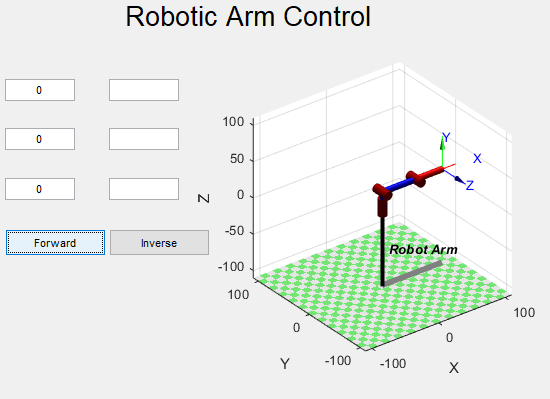
\includegraphics[width=0.8\columnwidth]{figures/robotarm1.png}
\end{center}
\caption{RRR Arm Model with all Joints at \ang{0}}
\label{fig:robotarm1}
\end{figure}

\begin{itemize}
\item Joint 1: Allows for 90 degrees of motion in the Y-Z Plane
\item Joint 2: Allows for 90 degrees of motion in the Y-Z Plane
\item Joint 3: Allows for 90 degrees of motion in the X-Y Plane
\end{itemize}

\begin{figure}
\begin{center}
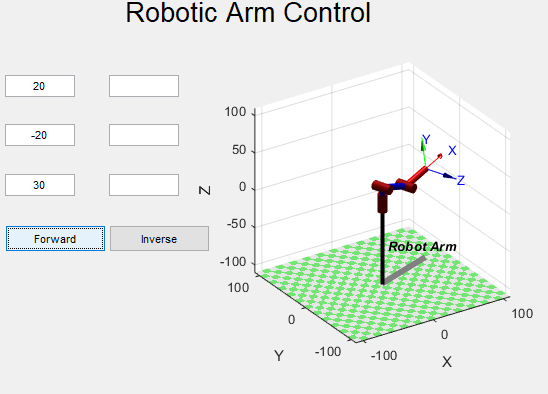
\includegraphics[width=0.8\columnwidth]{figures/robotarm2.png}
\end{center}
\caption{RRR Arm in Alternate Position}
\label{fig:robotarm2}
\end{figure}

\subsection{Torque}
The Average torque for a servo running at \SI{6}{\volt} is \SI{0.988}{\newton\meter}. The plants we are working with will be light in weight and the arm will not have a problem with torque in carrying the plants. This was concluded through testing with the prototype arm we built. We used heavy metal pieces from the EW202 classroom and the arm still moved very well.

\begin{figure}
\begin{center}
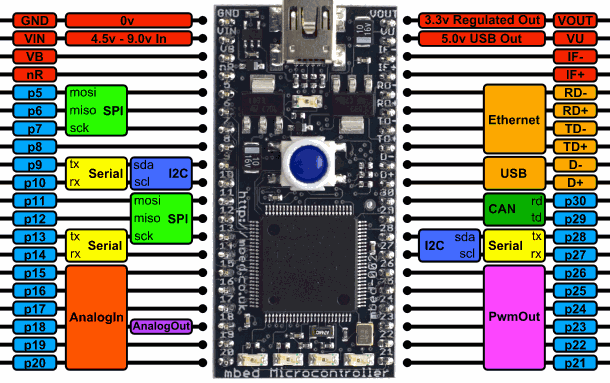
\includegraphics[width=\columnwidth]{figures/robotarm3.png}
\end{center}
\caption{Mbed Pinout}
\label{fig:robotarm3}
\end{figure}

\subsection{Mbed Configuration}
The Mbed will be on top of the drone body frame. The pins used for servo control are \lstinline{p21}, \lstinline{p22}, and \lstinline{p23} for \lstinline{PwmOut}. Commands for the Mbed can be sent through Teraterm or a Matlab User Interface. 

\subsection{Camera}
There must be an additional camera placed near the base of the robot arm so the user can see what the arm is doing in real time. We were thinking of the GoPro Hero Session because of its small size and quality. 

\subsection{Biggest Challenges}
We have not done any testing on how telemetry will work between the User’s computer and the Mbed, so that is a problem we are still facing. Example code for Mbed telemetry can be found online and I added one in this folder. Another option if telemetry is deemed overkill is an Mbed specific wireless transceiver called the nRF24L01. It could be used for sending video data and commands from the user wirelessly, but it only has a range of \SI{100}{\meter}. Another option is and Xbee capable of long range wireless communication.

We need testing on if a \SI{6}{\volt} battery will be enough to power the Mbed and all three servos. 

We need testing on the best place to place the additional camera and how to connect it to the Mbed and then to the user.